\documentclass[a4paper]{book}
\usepackage{a4wide}
\usepackage{makeidx}
\usepackage{graphicx}
\usepackage{multicol}
\usepackage{float}
\usepackage{listings}
\usepackage{color}
\usepackage{textcomp}
\usepackage{alltt}
\usepackage{times}
\usepackage{ifpdf}
\ifpdf
\usepackage[pdftex,
            pagebackref=true,
            colorlinks=true,
            linkcolor=blue,
            unicode
           ]{hyperref}
\else
\usepackage[ps2pdf,
            pagebackref=true,
            colorlinks=true,
            linkcolor=blue,
            unicode
           ]{hyperref}
\usepackage{pspicture}
\fi
\usepackage[utf8]{inputenc}
\usepackage{doxygen}
\lstset{language=C++,inputencoding=utf8,basicstyle=\footnotesize,breaklines=true,breakatwhitespace=true,tabsize=8,numbers=left }
\makeindex
\setcounter{tocdepth}{3}
\renewcommand{\footrulewidth}{0.4pt}
\begin{document}
\hypersetup{pageanchor=false}
\begin{titlepage}
\vspace*{7cm}
\begin{center}
{\Large RInside }\\
\vspace*{1cm}
{\large Generated by Doxygen 1.6.1}\\
\vspace*{0.5cm}
{\small Sat Sep 12 12:33:46 2009}\\
\end{center}
\end{titlepage}
\clearemptydoublepage
\pagenumbering{roman}
\tableofcontents
\clearemptydoublepage
\pagenumbering{arabic}
\hypersetup{pageanchor=true}
\chapter{Class Index}
\section{Class List}
Here are the classes, structs, unions and interfaces with brief descriptions:\begin{DoxyCompactList}
\item\contentsline{section}{\hyperlink{classMemBuf}{MemBuf} }{\pageref{classMemBuf}}{}
\item\contentsline{section}{\hyperlink{structMemBuf_1_1membuf__st}{MemBuf::membuf\_\-st} }{\pageref{structMemBuf_1_1membuf__st}}{}
\item\contentsline{section}{\hyperlink{classRInside}{RInside} }{\pageref{classRInside}}{}
\end{DoxyCompactList}

\chapter{File Index}
\section{File List}
Here is a list of all files with brief descriptions:\begin{DoxyCompactList}
\item\contentsline{section}{src/\hyperlink{MemBuf_8cpp}{MemBuf.cpp} }{\pageref{MemBuf_8cpp}}{}
\item\contentsline{section}{src/\hyperlink{MemBuf_8h}{MemBuf.h} }{\pageref{MemBuf_8h}}{}
\item\contentsline{section}{src/\hyperlink{RInside_8cpp}{RInside.cpp} }{\pageref{RInside_8cpp}}{}
\item\contentsline{section}{src/\hyperlink{RInside_8h}{RInside.h} }{\pageref{RInside_8h}}{}
\end{DoxyCompactList}

\chapter{Class Documentation}
\hypertarget{classMemBuf}{
\section{MemBuf Class Reference}
\label{classMemBuf}\index{MemBuf@{MemBuf}}
}


{\ttfamily \#include $<$MemBuf.h$>$}Collaboration diagram for MemBuf:\nopagebreak
\begin{figure}[H]
\begin{center}
\leavevmode
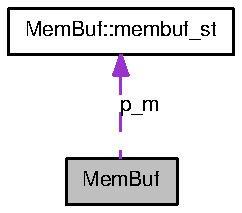
\includegraphics[width=152pt]{classMemBuf__coll__graph}
\end{center}
\end{figure}
\subsection*{Classes}
\begin{DoxyCompactItemize}
\item 
struct \hyperlink{structMemBuf_1_1membuf__st}{membuf\_\-st}
\end{DoxyCompactItemize}
\subsection*{Public Member Functions}
\begin{DoxyCompactItemize}
\item 
\hyperlink{classMemBuf_ae5cd261b2167fdb718e795ecee5e131d}{MemBuf} (int sizebytes=1024)
\item 
\hyperlink{classMemBuf_a84884d61f69e047814a365e8f0053829}{$\sim$MemBuf} ()
\item 
void \hyperlink{classMemBuf_a4cb3b44d88059c382184ca7d1aa1f235}{resize} ()
\item 
void \hyperlink{classMemBuf_acecce3962e522cdcabba571ffd51f940}{rewind} ()
\item 
void \hyperlink{classMemBuf_a98a5b5de27fb73dd3433773b825faf21}{add} (char $\ast$buf)
\item 
unsigned char $\ast$ \hyperlink{classMemBuf_a910edfa13107da037c7ccfc80adc0243}{getBufPtr} ()
\end{DoxyCompactItemize}
\subsection*{Private Types}
\begin{DoxyCompactItemize}
\item 
typedef struct \hyperlink{structMemBuf_1_1membuf__st}{MemBuf::membuf\_\-st} $\ast$ \hyperlink{classMemBuf_a36106702ece9c5960a6e1bd670dcea5e}{membuf\_\-t}
\end{DoxyCompactItemize}
\subsection*{Private Attributes}
\begin{DoxyCompactItemize}
\item 
\hyperlink{structMemBuf_1_1membuf__st}{membuf\_\-t} \hyperlink{classMemBuf_a2082ceb5554215dd792a83b2679a805a}{p\_\-m}
\end{DoxyCompactItemize}


\subsection{Detailed Description}


Definition at line 7 of file MemBuf.h.

\subsection{Member Typedef Documentation}
\hypertarget{classMemBuf_a36106702ece9c5960a6e1bd670dcea5e}{
\index{MemBuf@{MemBuf}!membuf\_\-t@{membuf\_\-t}}
\index{membuf\_\-t@{membuf\_\-t}!MemBuf@{MemBuf}}
\subsubsection[{membuf\_\-t}]{\setlength{\rightskip}{0pt plus 5cm}typedef struct {\bf MemBuf::membuf\_\-st} $\ast$ {\bf MemBuf::membuf\_\-t}\hspace{0.3cm}{\ttfamily  \mbox{[}private\mbox{]}}}}
\label{classMemBuf_a36106702ece9c5960a6e1bd670dcea5e}


\subsection{Constructor \& Destructor Documentation}
\hypertarget{classMemBuf_ae5cd261b2167fdb718e795ecee5e131d}{
\index{MemBuf@{MemBuf}!MemBuf@{MemBuf}}
\index{MemBuf@{MemBuf}!MemBuf@{MemBuf}}
\subsubsection[{MemBuf}]{\setlength{\rightskip}{0pt plus 5cm}MemBuf::MemBuf (int {\em sizebytes} = {\ttfamily 1024})}}
\label{classMemBuf_ae5cd261b2167fdb718e795ecee5e131d}


Definition at line 22 of file MemBuf.cpp.

References MemBuf::membuf\_\-st::buf, MemBuf::membuf\_\-st::count, p\_\-m, programName, MemBuf::membuf\_\-st::size, and verbose.\hypertarget{classMemBuf_a84884d61f69e047814a365e8f0053829}{
\index{MemBuf@{MemBuf}!$\sim$MemBuf@{$\sim$MemBuf}}
\index{$\sim$MemBuf@{$\sim$MemBuf}!MemBuf@{MemBuf}}
\subsubsection[{$\sim$MemBuf}]{\setlength{\rightskip}{0pt plus 5cm}MemBuf::$\sim$MemBuf ()}}
\label{classMemBuf_a84884d61f69e047814a365e8f0053829}


Definition at line 16 of file MemBuf.cpp.

References p\_\-m, and verbose.

\subsection{Member Function Documentation}
\hypertarget{classMemBuf_a98a5b5de27fb73dd3433773b825faf21}{
\index{MemBuf@{MemBuf}!add@{add}}
\index{add@{add}!MemBuf@{MemBuf}}
\subsubsection[{add}]{\setlength{\rightskip}{0pt plus 5cm}void MemBuf::add (char $\ast$ {\em buf})}}
\label{classMemBuf_a98a5b5de27fb73dd3433773b825faf21}


Definition at line 54 of file MemBuf.cpp.

References MemBuf::membuf\_\-st::buf, MemBuf::membuf\_\-st::count, p\_\-m, resize(), and MemBuf::membuf\_\-st::size.

Referenced by RInside::parseEval().

Here is the call graph for this function:\nopagebreak
\begin{figure}[H]
\begin{center}
\leavevmode
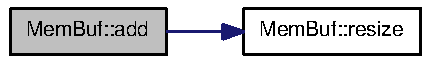
\includegraphics[width=121pt]{classMemBuf_a98a5b5de27fb73dd3433773b825faf21_cgraph}
\end{center}
\end{figure}
\hypertarget{classMemBuf_a910edfa13107da037c7ccfc80adc0243}{
\index{MemBuf@{MemBuf}!getBufPtr@{getBufPtr}}
\index{getBufPtr@{getBufPtr}!MemBuf@{MemBuf}}
\subsubsection[{getBufPtr}]{\setlength{\rightskip}{0pt plus 5cm}unsigned char$\ast$ MemBuf::getBufPtr ()\hspace{0.3cm}{\ttfamily  \mbox{[}inline\mbox{]}}}}
\label{classMemBuf_a910edfa13107da037c7ccfc80adc0243}


Definition at line 21 of file MemBuf.h.

References MemBuf::membuf\_\-st::buf, and p\_\-m.

Referenced by RInside::parseEval().\hypertarget{classMemBuf_a4cb3b44d88059c382184ca7d1aa1f235}{
\index{MemBuf@{MemBuf}!resize@{resize}}
\index{resize@{resize}!MemBuf@{MemBuf}}
\subsubsection[{resize}]{\setlength{\rightskip}{0pt plus 5cm}void MemBuf::resize ()}}
\label{classMemBuf_a4cb3b44d88059c382184ca7d1aa1f235}


Definition at line 39 of file MemBuf.cpp.

References MemBuf::membuf\_\-st::buf, p\_\-m, programName, and MemBuf::membuf\_\-st::size.

Referenced by add().\hypertarget{classMemBuf_acecce3962e522cdcabba571ffd51f940}{
\index{MemBuf@{MemBuf}!rewind@{rewind}}
\index{rewind@{rewind}!MemBuf@{MemBuf}}
\subsubsection[{rewind}]{\setlength{\rightskip}{0pt plus 5cm}void MemBuf::rewind ()}}
\label{classMemBuf_acecce3962e522cdcabba571ffd51f940}


Definition at line 50 of file MemBuf.cpp.

References MemBuf::membuf\_\-st::count, and p\_\-m.

Referenced by RInside::parseEval().

\subsection{Member Data Documentation}
\hypertarget{classMemBuf_a2082ceb5554215dd792a83b2679a805a}{
\index{MemBuf@{MemBuf}!p\_\-m@{p\_\-m}}
\index{p\_\-m@{p\_\-m}!MemBuf@{MemBuf}}
\subsubsection[{p\_\-m}]{\setlength{\rightskip}{0pt plus 5cm}{\bf membuf\_\-t} {\bf MemBuf::p\_\-m}\hspace{0.3cm}{\ttfamily  \mbox{[}private\mbox{]}}}}
\label{classMemBuf_a2082ceb5554215dd792a83b2679a805a}


Definition at line 14 of file MemBuf.h.

Referenced by add(), getBufPtr(), MemBuf(), resize(), rewind(), and $\sim$MemBuf().

The documentation for this class was generated from the following files:\begin{DoxyCompactItemize}
\item 
src/\hyperlink{MemBuf_8h}{MemBuf.h}\item 
src/\hyperlink{MemBuf_8cpp}{MemBuf.cpp}\end{DoxyCompactItemize}

\hypertarget{structMemBuf_1_1membuf__st}{
\section{MemBuf::membuf\_\-st Struct Reference}
\label{structMemBuf_1_1membuf__st}\index{MemBuf::membuf\_\-st@{MemBuf::membuf\_\-st}}
}
\subsection*{Public Attributes}
\begin{DoxyCompactItemize}
\item 
int \hyperlink{structMemBuf_1_1membuf__st_a5ee474be75ca5d65fce37f464d249535}{size}
\item 
int \hyperlink{structMemBuf_1_1membuf__st_a897938924fdb92f31dbaa9e494953248}{count}
\item 
unsigned char $\ast$ \hyperlink{structMemBuf_1_1membuf__st_acf4fd68d12e2d0b2ff8c4e526e6b9525}{buf}
\end{DoxyCompactItemize}


\subsection{Detailed Description}


Definition at line 9 of file MemBuf.h.

\subsection{Member Data Documentation}
\hypertarget{structMemBuf_1_1membuf__st_acf4fd68d12e2d0b2ff8c4e526e6b9525}{
\index{MemBuf::membuf\_\-st@{MemBuf::membuf\_\-st}!buf@{buf}}
\index{buf@{buf}!MemBuf::membuf_st@{MemBuf::membuf\_\-st}}
\subsubsection[{buf}]{\setlength{\rightskip}{0pt plus 5cm}unsigned char$\ast$ {\bf MemBuf::membuf\_\-st::buf}}}
\label{structMemBuf_1_1membuf__st_acf4fd68d12e2d0b2ff8c4e526e6b9525}


Definition at line 12 of file MemBuf.h.

Referenced by MemBuf::add(), MemBuf::getBufPtr(), MemBuf::MemBuf(), and MemBuf::resize().\hypertarget{structMemBuf_1_1membuf__st_a897938924fdb92f31dbaa9e494953248}{
\index{MemBuf::membuf\_\-st@{MemBuf::membuf\_\-st}!count@{count}}
\index{count@{count}!MemBuf::membuf_st@{MemBuf::membuf\_\-st}}
\subsubsection[{count}]{\setlength{\rightskip}{0pt plus 5cm}int {\bf MemBuf::membuf\_\-st::count}}}
\label{structMemBuf_1_1membuf__st_a897938924fdb92f31dbaa9e494953248}


Definition at line 11 of file MemBuf.h.

Referenced by MemBuf::add(), MemBuf::MemBuf(), and MemBuf::rewind().\hypertarget{structMemBuf_1_1membuf__st_a5ee474be75ca5d65fce37f464d249535}{
\index{MemBuf::membuf\_\-st@{MemBuf::membuf\_\-st}!size@{size}}
\index{size@{size}!MemBuf::membuf_st@{MemBuf::membuf\_\-st}}
\subsubsection[{size}]{\setlength{\rightskip}{0pt plus 5cm}int {\bf MemBuf::membuf\_\-st::size}}}
\label{structMemBuf_1_1membuf__st_a5ee474be75ca5d65fce37f464d249535}


Definition at line 10 of file MemBuf.h.

Referenced by MemBuf::add(), MemBuf::MemBuf(), and MemBuf::resize().

The documentation for this struct was generated from the following file:\begin{DoxyCompactItemize}
\item 
src/\hyperlink{MemBuf_8h}{MemBuf.h}\end{DoxyCompactItemize}

\hypertarget{classRInside}{
\section{RInside Class Reference}
\label{classRInside}\index{RInside@{RInside}}
}


{\ttfamily \#include $<$RInside.h$>$}Collaboration diagram for RInside:\nopagebreak
\begin{figure}[H]
\begin{center}
\leavevmode
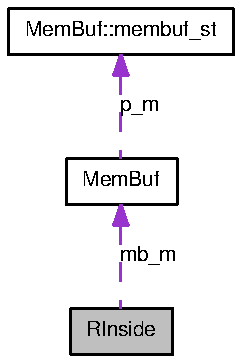
\includegraphics[width=152pt]{classRInside__coll__graph}
\end{center}
\end{figure}
\subsection*{Public Member Functions}
\begin{DoxyCompactItemize}
\item 
int \hyperlink{classRInside_a4cf10e78fb73bfda699f921c28e6b985}{parseEval} (const std::string \&line, SEXP \&ans)
\item 
int \hyperlink{classRInside_a9f18dc5011e1e32a52360b3d88f9bab7}{parseEvalQ} (const std::string \&line)
\item 
void \hyperlink{classRInside_aedd5db3eb2bcc97a93914088d599c8b4}{assign} (const std::vector$<$ std::vector$<$ double $>$ $>$ \&mat, const std::string \&nam)
\item 
void \hyperlink{classRInside_abae6700c75661cfb635859ac3d3c50d1}{assign} (const std::vector$<$ std::vector$<$ int $>$ $>$ \&mat, const std::string \&nam)
\item 
void \hyperlink{classRInside_a7c5cb94cc703541037e6acf243dc2b1b}{assign} (const std::vector$<$ std::string $>$ \&vec, const std::string \&nam)
\item 
void \hyperlink{classRInside_a9086ea21bd4a47d9411c6451c1ae50f5}{assign} (const std::vector$<$ double $>$ \&vec, const std::string \&nam)
\item 
void \hyperlink{classRInside_ab13e05865dec061ba1def1d922d2a58c}{assign} (const std::vector$<$ int $>$ \&vec, const std::string \&nam)
\item 
void \hyperlink{classRInside_a7073300c48c03478361b881e2d307ad6}{assign} (const std::string \&txt, const std::string \&nam)
\item 
\hyperlink{classRInside_aeecbfd63737539d1731b2f38852b3751}{RInside} (const int argc, const char $\ast$const argv\mbox{[}$\,$\mbox{]})
\item 
\hyperlink{classRInside_a277fc333d12163eaea9b903711586146}{$\sim$RInside} ()
\end{DoxyCompactItemize}
\subsection*{Private Member Functions}
\begin{DoxyCompactItemize}
\item 
void \hyperlink{classRInside_ae045f7e3d8b0881e2af8cdfb5c5fc118}{init\_\-tempdir} (void)
\item 
void \hyperlink{classRInside_af9920dd157552b7a5dce8573574ce78d}{init\_\-rand} (void)
\item 
void \hyperlink{classRInside_a41c250f2ef249a02a0d32e761628d943}{autoloads} (void)
\end{DoxyCompactItemize}
\subsection*{Private Attributes}
\begin{DoxyCompactItemize}
\item 
\hyperlink{classMemBuf}{MemBuf} \hyperlink{classRInside_ad078e52002a242f7f5c94211ca3dd8be}{mb\_\-m}
\item 
bool \hyperlink{classRInside_a186dad3e463fedc586f3d02784a814b2}{verbose\_\-m}
\end{DoxyCompactItemize}


\subsection{Detailed Description}


Definition at line 21 of file RInside.h.

\subsection{Constructor \& Destructor Documentation}
\hypertarget{classRInside_aeecbfd63737539d1731b2f38852b3751}{
\index{RInside@{RInside}!RInside@{RInside}}
\index{RInside@{RInside}!RInside@{RInside}}
\subsubsection[{RInside}]{\setlength{\rightskip}{0pt plus 5cm}RInside::RInside (const int {\em argc}, \/  const char $\ast$const  {\em argv}\mbox{[}$\,$\mbox{]})}}
\label{classRInside_aeecbfd63737539d1731b2f38852b3751}


Definition at line 20 of file RInside.cpp.

References autoloads(), init\_\-rand(), init\_\-tempdir(), programName, verbose, and verbose\_\-m.

Here is the call graph for this function:\nopagebreak
\begin{figure}[H]
\begin{center}
\leavevmode
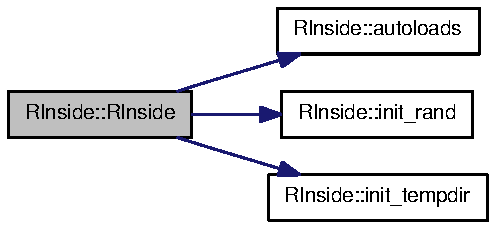
\includegraphics[width=137pt]{classRInside_aeecbfd63737539d1731b2f38852b3751_cgraph}
\end{center}
\end{figure}
\hypertarget{classRInside_a277fc333d12163eaea9b903711586146}{
\index{RInside@{RInside}!$\sim$RInside@{$\sim$RInside}}
\index{$\sim$RInside@{$\sim$RInside}!RInside@{RInside}}
\subsubsection[{$\sim$RInside}]{\setlength{\rightskip}{0pt plus 5cm}RInside::$\sim$RInside ()}}
\label{classRInside_a277fc333d12163eaea9b903711586146}


Definition at line 14 of file RInside.cpp.

References verbose.

\subsection{Member Function Documentation}
\hypertarget{classRInside_a7073300c48c03478361b881e2d307ad6}{
\index{RInside@{RInside}!assign@{assign}}
\index{assign@{assign}!RInside@{RInside}}
\subsubsection[{assign}]{\setlength{\rightskip}{0pt plus 5cm}void RInside::assign (const std::string \& {\em txt}, \/  const std::string \& {\em nam})}}
\label{classRInside_a7073300c48c03478361b881e2d307ad6}


Definition at line 308 of file RInside.cpp.\hypertarget{classRInside_ab13e05865dec061ba1def1d922d2a58c}{
\index{RInside@{RInside}!assign@{assign}}
\index{assign@{assign}!RInside@{RInside}}
\subsubsection[{assign}]{\setlength{\rightskip}{0pt plus 5cm}void RInside::assign (const std::vector$<$ int $>$ \& {\em vec}, \/  const std::string \& {\em nam})}}
\label{classRInside_ab13e05865dec061ba1def1d922d2a58c}


Definition at line 298 of file RInside.cpp.\hypertarget{classRInside_a9086ea21bd4a47d9411c6451c1ae50f5}{
\index{RInside@{RInside}!assign@{assign}}
\index{assign@{assign}!RInside@{RInside}}
\subsubsection[{assign}]{\setlength{\rightskip}{0pt plus 5cm}void RInside::assign (const std::vector$<$ double $>$ \& {\em vec}, \/  const std::string \& {\em nam})}}
\label{classRInside_a9086ea21bd4a47d9411c6451c1ae50f5}


Definition at line 275 of file RInside.cpp.\hypertarget{classRInside_a7c5cb94cc703541037e6acf243dc2b1b}{
\index{RInside@{RInside}!assign@{assign}}
\index{assign@{assign}!RInside@{RInside}}
\subsubsection[{assign}]{\setlength{\rightskip}{0pt plus 5cm}void RInside::assign (const std::vector$<$ std::string $>$ \& {\em vec}, \/  const std::string \& {\em nam})}}
\label{classRInside_a7c5cb94cc703541037e6acf243dc2b1b}


Definition at line 286 of file RInside.cpp.\hypertarget{classRInside_abae6700c75661cfb635859ac3d3c50d1}{
\index{RInside@{RInside}!assign@{assign}}
\index{assign@{assign}!RInside@{RInside}}
\subsubsection[{assign}]{\setlength{\rightskip}{0pt plus 5cm}void RInside::assign (const std::vector$<$ std::vector$<$ int $>$ $>$ \& {\em mat}, \/  const std::string \& {\em nam})}}
\label{classRInside_abae6700c75661cfb635859ac3d3c50d1}


Definition at line 261 of file RInside.cpp.\hypertarget{classRInside_aedd5db3eb2bcc97a93914088d599c8b4}{
\index{RInside@{RInside}!assign@{assign}}
\index{assign@{assign}!RInside@{RInside}}
\subsubsection[{assign}]{\setlength{\rightskip}{0pt plus 5cm}void RInside::assign (const std::vector$<$ std::vector$<$ double $>$ $>$ \& {\em mat}, \/  const std::string \& {\em nam})}}
\label{classRInside_aedd5db3eb2bcc97a93914088d599c8b4}


Definition at line 247 of file RInside.cpp.\hypertarget{classRInside_a41c250f2ef249a02a0d32e761628d943}{
\index{RInside@{RInside}!autoloads@{autoloads}}
\index{autoloads@{autoloads}!RInside@{RInside}}
\subsubsection[{autoloads}]{\setlength{\rightskip}{0pt plus 5cm}void RInside::autoloads (void)\hspace{0.3cm}{\ttfamily  \mbox{[}private\mbox{]}}}}
\label{classRInside_a41c250f2ef249a02a0d32e761628d943}


Definition at line 102 of file RInside.cpp.

References programName.

Referenced by RInside().\hypertarget{classRInside_af9920dd157552b7a5dce8573574ce78d}{
\index{RInside@{RInside}!init\_\-rand@{init\_\-rand}}
\index{init\_\-rand@{init\_\-rand}!RInside@{RInside}}
\subsubsection[{init\_\-rand}]{\setlength{\rightskip}{0pt plus 5cm}void RInside::init\_\-rand (void)\hspace{0.3cm}{\ttfamily  \mbox{[}private\mbox{]}}}}
\label{classRInside_af9920dd157552b7a5dce8573574ce78d}


Definition at line 93 of file RInside.cpp.

Referenced by RInside().\hypertarget{classRInside_ae045f7e3d8b0881e2af8cdfb5c5fc118}{
\index{RInside@{RInside}!init\_\-tempdir@{init\_\-tempdir}}
\index{init\_\-tempdir@{init\_\-tempdir}!RInside@{RInside}}
\subsubsection[{init\_\-tempdir}]{\setlength{\rightskip}{0pt plus 5cm}void RInside::init\_\-tempdir (void)\hspace{0.3cm}{\ttfamily  \mbox{[}private\mbox{]}}}}
\label{classRInside_ae045f7e3d8b0881e2af8cdfb5c5fc118}


Definition at line 74 of file RInside.cpp.

Referenced by RInside().\hypertarget{classRInside_a4cf10e78fb73bfda699f921c28e6b985}{
\index{RInside@{RInside}!parseEval@{parseEval}}
\index{parseEval@{parseEval}!RInside@{RInside}}
\subsubsection[{parseEval}]{\setlength{\rightskip}{0pt plus 5cm}int RInside::parseEval (const std::string \& {\em line}, \/  SEXP \& {\em ans})}}
\label{classRInside_a4cf10e78fb73bfda699f921c28e6b985}


Definition at line 193 of file RInside.cpp.

References MemBuf::add(), MemBuf::getBufPtr(), mb\_\-m, programName, MemBuf::rewind(), and verbose\_\-m.

Referenced by parseEvalQ().

Here is the call graph for this function:\nopagebreak
\begin{figure}[H]
\begin{center}
\leavevmode
\includegraphics[width=200pt]{classRInside_a4cf10e78fb73bfda699f921c28e6b985_cgraph}
\end{center}
\end{figure}
\hypertarget{classRInside_a9f18dc5011e1e32a52360b3d88f9bab7}{
\index{RInside@{RInside}!parseEvalQ@{parseEvalQ}}
\index{parseEvalQ@{parseEvalQ}!RInside@{RInside}}
\subsubsection[{parseEvalQ}]{\setlength{\rightskip}{0pt plus 5cm}int RInside::parseEvalQ (const std::string \& {\em line})}}
\label{classRInside_a9f18dc5011e1e32a52360b3d88f9bab7}


Definition at line 240 of file RInside.cpp.

References parseEval().

Here is the call graph for this function:\nopagebreak
\begin{figure}[H]
\begin{center}
\leavevmode
\includegraphics[width=271pt]{classRInside_a9f18dc5011e1e32a52360b3d88f9bab7_cgraph}
\end{center}
\end{figure}


\subsection{Member Data Documentation}
\hypertarget{classRInside_ad078e52002a242f7f5c94211ca3dd8be}{
\index{RInside@{RInside}!mb\_\-m@{mb\_\-m}}
\index{mb\_\-m@{mb\_\-m}!RInside@{RInside}}
\subsubsection[{mb\_\-m}]{\setlength{\rightskip}{0pt plus 5cm}{\bf MemBuf} {\bf RInside::mb\_\-m}\hspace{0.3cm}{\ttfamily  \mbox{[}private\mbox{]}}}}
\label{classRInside_ad078e52002a242f7f5c94211ca3dd8be}


Definition at line 23 of file RInside.h.

Referenced by parseEval().\hypertarget{classRInside_a186dad3e463fedc586f3d02784a814b2}{
\index{RInside@{RInside}!verbose\_\-m@{verbose\_\-m}}
\index{verbose\_\-m@{verbose\_\-m}!RInside@{RInside}}
\subsubsection[{verbose\_\-m}]{\setlength{\rightskip}{0pt plus 5cm}bool {\bf RInside::verbose\_\-m}\hspace{0.3cm}{\ttfamily  \mbox{[}private\mbox{]}}}}
\label{classRInside_a186dad3e463fedc586f3d02784a814b2}


Definition at line 25 of file RInside.h.

Referenced by parseEval(), and RInside().

The documentation for this class was generated from the following files:\begin{DoxyCompactItemize}
\item 
src/\hyperlink{RInside_8h}{RInside.h}\item 
src/\hyperlink{RInside_8cpp}{RInside.cpp}\end{DoxyCompactItemize}

\chapter{File Documentation}
\hypertarget{MemBuf_8cpp}{
\section{src/MemBuf.cpp File Reference}
\label{MemBuf_8cpp}\index{src/MemBuf.cpp@{src/MemBuf.cpp}}
}
{\ttfamily \#include $<$iostream$>$}\par
{\ttfamily \#include $<$cstdlib$>$}\par
{\ttfamily \#include $<$cstring$>$}\par
{\ttfamily \#include \char`\"{}MemBuf.h\char`\"{}}\par
Include dependency graph for MemBuf.cpp:\nopagebreak
\begin{figure}[H]
\begin{center}
\leavevmode
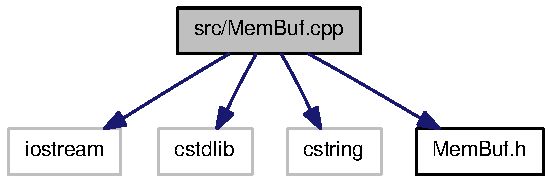
\includegraphics[width=150pt]{MemBuf_8cpp__incl}
\end{center}
\end{figure}
\subsection*{Variables}
\begin{DoxyCompactItemize}
\item 
bool \hyperlink{MemBuf_8cpp_ab3f078684998b83967d507d0f453f454}{verbose}
\item 
const char $\ast$ \hyperlink{MemBuf_8cpp_a1afa8960a291d0a8287ea6ab84d0078c}{programName}
\end{DoxyCompactItemize}


\subsection{Variable Documentation}
\hypertarget{MemBuf_8cpp_a1afa8960a291d0a8287ea6ab84d0078c}{
\index{MemBuf.cpp@{MemBuf.cpp}!programName@{programName}}
\index{programName@{programName}!MemBuf.cpp@{MemBuf.cpp}}
\subsubsection[{programName}]{\setlength{\rightskip}{0pt plus 5cm}const char$\ast$ {\bf programName}}}
\label{MemBuf_8cpp_a1afa8960a291d0a8287ea6ab84d0078c}


Definition at line 12 of file RInside.cpp.

Referenced by RInside::autoloads(), MemBuf::MemBuf(), RInside::parseEval(), MemBuf::resize(), and RInside::RInside().\hypertarget{MemBuf_8cpp_ab3f078684998b83967d507d0f453f454}{
\index{MemBuf.cpp@{MemBuf.cpp}!verbose@{verbose}}
\index{verbose@{verbose}!MemBuf.cpp@{MemBuf.cpp}}
\subsubsection[{verbose}]{\setlength{\rightskip}{0pt plus 5cm}bool {\bf verbose}}}
\label{MemBuf_8cpp_ab3f078684998b83967d507d0f453f454}


Definition at line 11 of file RInside.cpp.

Referenced by MemBuf::MemBuf(), RInside::RInside(), MemBuf::$\sim$MemBuf(), and RInside::$\sim$RInside().
\hypertarget{MemBuf_8h}{
\section{src/MemBuf.h File Reference}
\label{MemBuf_8h}\index{src/MemBuf.h@{src/MemBuf.h}}
}
This graph shows which files directly or indirectly include this file:\nopagebreak
\begin{figure}[H]
\begin{center}
\leavevmode
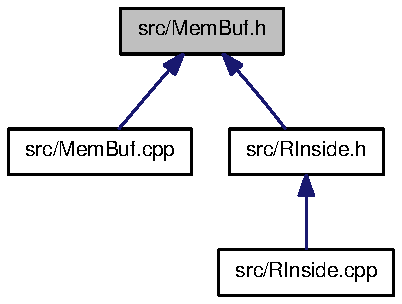
\includegraphics[width=114pt]{MemBuf_8h__dep__incl}
\end{center}
\end{figure}
\subsection*{Classes}
\begin{DoxyCompactItemize}
\item 
class \hyperlink{classMemBuf}{MemBuf}
\item 
struct \hyperlink{structMemBuf_1_1membuf__st}{MemBuf::membuf\_\-st}
\end{DoxyCompactItemize}

\hypertarget{RInside_8cpp}{
\section{src/RInside.cpp File Reference}
\label{RInside_8cpp}\index{src/RInside.cpp@{src/RInside.cpp}}
}
{\ttfamily \#include \char`\"{}RInside.h\char`\"{}}\par
{\ttfamily \#include $<$sys/time.h$>$}\par
{\ttfamily \#include \char`\"{}RInsideEnvVars.h\char`\"{}}\par
{\ttfamily \#include \char`\"{}RInsideAutoloads.h\char`\"{}}\par
Include dependency graph for RInside.cpp:\nopagebreak
\begin{figure}[H]
\begin{center}
\leavevmode
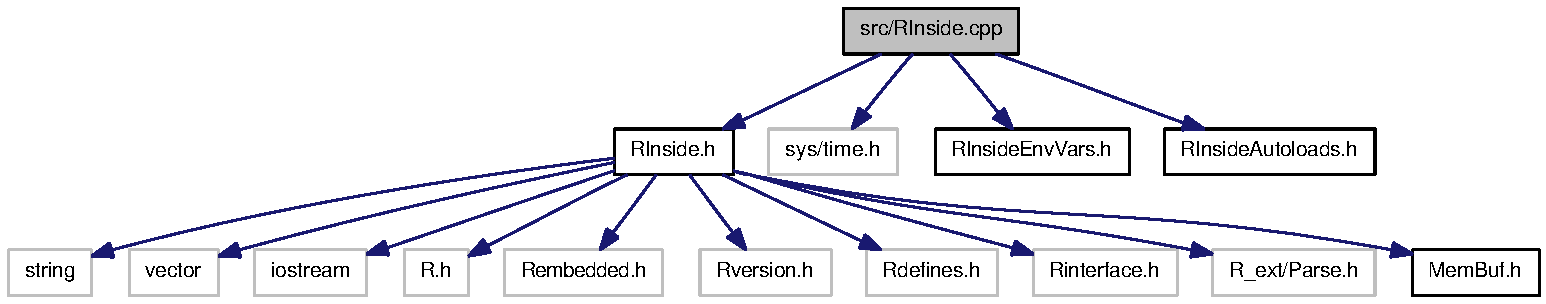
\includegraphics[width=389pt]{RInside_8cpp__incl}
\end{center}
\end{figure}
\subsection*{Variables}
\begin{DoxyCompactItemize}
\item 
bool \hyperlink{RInside_8cpp_ab3f078684998b83967d507d0f453f454}{verbose} = false
\item 
const char $\ast$ \hyperlink{RInside_8cpp_a1afa8960a291d0a8287ea6ab84d0078c}{programName} = \char`\"{}RInside\char`\"{}
\end{DoxyCompactItemize}


\subsection{Variable Documentation}
\hypertarget{RInside_8cpp_a1afa8960a291d0a8287ea6ab84d0078c}{
\index{RInside.cpp@{RInside.cpp}!programName@{programName}}
\index{programName@{programName}!RInside.cpp@{RInside.cpp}}
\subsubsection[{programName}]{\setlength{\rightskip}{0pt plus 5cm}const char$\ast$ {\bf programName} = \char`\"{}RInside\char`\"{}}}
\label{RInside_8cpp_a1afa8960a291d0a8287ea6ab84d0078c}


Definition at line 12 of file RInside.cpp.

Referenced by RInside::autoloads(), MemBuf::MemBuf(), RInside::parseEval(), MemBuf::resize(), and RInside::RInside().\hypertarget{RInside_8cpp_ab3f078684998b83967d507d0f453f454}{
\index{RInside.cpp@{RInside.cpp}!verbose@{verbose}}
\index{verbose@{verbose}!RInside.cpp@{RInside.cpp}}
\subsubsection[{verbose}]{\setlength{\rightskip}{0pt plus 5cm}bool {\bf verbose} = false}}
\label{RInside_8cpp_ab3f078684998b83967d507d0f453f454}


Definition at line 11 of file RInside.cpp.

Referenced by MemBuf::MemBuf(), RInside::RInside(), MemBuf::$\sim$MemBuf(), and RInside::$\sim$RInside().
\hypertarget{RInside_8h}{
\section{src/RInside.h File Reference}
\label{RInside_8h}\index{src/RInside.h@{src/RInside.h}}
}
{\ttfamily \#include $<$string$>$}\par
{\ttfamily \#include $<$vector$>$}\par
{\ttfamily \#include $<$iostream$>$}\par
{\ttfamily \#include $<$R.h$>$}\par
{\ttfamily \#include $<$Rembedded.h$>$}\par
{\ttfamily \#include $<$Rversion.h$>$}\par
{\ttfamily \#include $<$Rdefines.h$>$}\par
{\ttfamily \#include $<$Rinterface.h$>$}\par
{\ttfamily \#include $<$R\_\-ext/Parse.h$>$}\par
{\ttfamily \#include \char`\"{}MemBuf.h\char`\"{}}\par
Include dependency graph for RInside.h:\nopagebreak
\begin{figure}[H]
\begin{center}
\leavevmode
\includegraphics[width=389pt]{RInside_8h__incl}
\end{center}
\end{figure}
This graph shows which files directly or indirectly include this file:\nopagebreak
\begin{figure}[H]
\begin{center}
\leavevmode
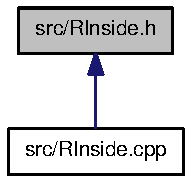
\includegraphics[width=64pt]{RInside_8h__dep__incl}
\end{center}
\end{figure}
\subsection*{Classes}
\begin{DoxyCompactItemize}
\item 
class \hyperlink{classRInside}{RInside}
\end{DoxyCompactItemize}
\subsection*{Defines}
\begin{DoxyCompactItemize}
\item 
\#define \hyperlink{RInside_8h_ad627310d56341e3150e8b86d6b88d6a2}{R\_\-INTERFACE\_\-PTRS}
\end{DoxyCompactItemize}


\subsection{Define Documentation}
\hypertarget{RInside_8h_ad627310d56341e3150e8b86d6b88d6a2}{
\index{RInside.h@{RInside.h}!R\_\-INTERFACE\_\-PTRS@{R\_\-INTERFACE\_\-PTRS}}
\index{R\_\-INTERFACE\_\-PTRS@{R\_\-INTERFACE\_\-PTRS}!RInside.h@{RInside.h}}
\subsubsection[{R\_\-INTERFACE\_\-PTRS}]{\setlength{\rightskip}{0pt plus 5cm}\#define R\_\-INTERFACE\_\-PTRS}}
\label{RInside_8h_ad627310d56341e3150e8b86d6b88d6a2}


Definition at line 15 of file RInside.h.
\printindex
\end{document}
